\chapter{第一代量子天文学科学案例}
\label{chap:e25}

\begin{chapteropening}
前面几个部分，我们像攒装备一样把工具一件件配齐了：复振幅与相位（第 \ref{chap:e01} 章）、带宽与相干时间（第 \ref{chap:e02} 章）、泊松与散粒噪声（第 \ref{chap:e03} 章）、二阶相干 \(g^{(2)}\) 与 Siegert 关系（第 \ref{chap:e08} 章）、强度干涉与 van Cittert--Zernike 定理（第 \ref{chap:e10} 章）、从可见度到成像（第 \ref{chap:e11} 章）、量子估计与 SPADE（第 \ref{chap:e12} 章）、事件表与时钟（第 \ref{chap:e13} 章）、误差预算（第 \ref{chap:e15} 章），一直到把恒星当成量子光源（第 \ref{chap:e17} 章）、把瞬变缝成多信使事件（第 \ref{chap:e20} 章）。装备齐了，就该下场打仗。本章要回答一个非常实际的问题：\textbf{在今天这套仪器条件下，第一代量子天文学到底能做哪些"现在就能做"的真科学？}我们会沿着一条清单走下去——亮星角直径、快速自转的扁球、密近双星、Be 星盘与 Wolf--Rayet 风、新星与 Type Ia 的膨胀、Crab 的光子统计、自然激光候选——每到一站都问同样三件事：\textbf{要测什么可观测量？需要什么样的阵列、曝光和精度？它能回答哪个天体物理问题？}这不是画大饼，而是把前面每一章的公式，落到明晚就能对准的目标上。
\end{chapteropening}

\section{给案例排序：亮度、角尺度、外部先验这三把尺子}
\label{sec:e25-triage}

打仗不能一拥而上。第一代项目最怕的不是"题目不够漂亮"，而是"漂亮题目却做不出结果"。所以在挑目标之前，先要建立一套冷静的排序法，让科学价值、技术可行性、失败后仍有产出这三件事同时进入判断。

\textbf{第一把尺子是亮度。}强度干涉（intensity interferometry）的信号是符合计数（coincidence），它的统计精度最终由攒到的\textbf{光子对数}决定（第 \ref{chap:e15} 章）。光子率越高，同样时间里攒的对数越多，误差按对数平方根往下掉。对当前这一代仪器，一个粗略的分区是：视星等 \(m_V\lesssim5\) 的热星是"验证区"，信号强、能反复复现；\(m_V\simeq6\text{--}7\) 是"有挑战但能规划"的区域；\(m_V\gtrsim9\) 通常就得靠更大阵列、多谱通道、更长积分或更低系统噪声才够得着。LeBohec 与 Holder 的估算给了一个可以记住的锚点：一对 \(100\,\mathrm{m^2}\)、电子带宽到 GHz 量级的望远镜，5 小时内可以对 \(m_V\simeq6.7\) 的源做到几倍标准差的相关检出 \citep{2006ApJ...649..399L,2013APh....43..331D}。

\textbf{第二把尺子是角尺度。}亮度决定"有没有光子"，角尺度决定"这些光子能不能变成参数"。第 \ref{chap:e11} 章讲过，一台基线为 \(B\)、波长为 \(\lambda\) 的干涉仪，能分辨的角尺度标度是 \(\lambda/B\)。若目标角尺度 \(\theta\gg\lambda/B\)，那么在长基线上平方可见度 \(|V|^2\) 已经掉到接近零，只有短基线还剩信号；若 \(\theta\ll\lambda/B\)，则所有基线都看到一个"未解析的点"，可见度对直径的导数几乎为零，测了也约束不动参数。两头都不好，最舒服的是让主要结构正好落在你手上的基线区间里——对现有 IACT 阵列是 \(50\text{--}300\,\mathrm{m}\)，对未来 CTA 型阵列是 \(0.5\text{--}2\,\mathrm{km}\)。

\textbf{第三把尺子是外部先验。}同样几个 \(|V|^2\) 数据点，如果你事先知道距离、光谱、轨道、径向速度或一个理论大气模型，它们就能被"翻译"成真正的物理参数；如果什么先验都没有，几个孤零零的可见度点往往互相退化，谁也钉不住谁。所以有成熟先验的目标，天然排在前面 \citep{2003RPPh...66..789M,2012MNRAS.419..172N}。

把这三把尺子写成一个可以打分的排序式，就得到一个实用的分诊（triage）工具：
\begin{equation}
  \mathcal P
  =
  \frac{
  W_{\rm sci}\,
  R_{\rm tech}\,
  R_{\rm prior}
  }{
  1+R_{\rm sys}+R_{\rm trigger}
  } .
  \label{eq:e25-priority-score}
\end{equation}
\begin{formulaexplain}
\(\mathcal P\) 是项目排序分数。分子上，科学回报 \(W_{\rm sci}\)、技术成熟度 \(R_{\rm tech}\)、外部先验 \(R_{\rm prior}\) 越高分越高；分母上，系统误差风险 \(R_{\rm sys}\)、触发/调度风险 \(R_{\rm trigger}\) 越高分越低。它专门用来防止"只凭题目好听"就上马。
\end{formulaexplain}
逐项落地：\(W_{\rm sci}\) 是科学回报（这个结果有多重要），\(R_{\rm tech}\) 是技术成熟度（现有仪器能不能稳定做出来），\(R_{\rm prior}\) 是外部先验与模型可解释性，\(R_{\rm sys}\) 是系统误差风险（零基线相关、时间同步、背景扣除有多容易翻车），\(R_{\rm trigger}\) 是触发与调度风险（要不要抢时间窗、能不能随时开机）。这些量都无量纲，实际使用时只需粗分几档（高/中/低），目的不是算出一个精确小数，而是\textbf{不让单一维度支配选择}。举个对照：Type Ia 的几何距离 \(W_{\rm sci}\) 极高，可它的 \(R_{\rm trigger}\) 和 \(R_{\rm sys}\) 也高，分母被顶起来，第一代不宜强上；亮星角直径的 \(W_{\rm sci}\) 只是中等，却有很高的 \(R_{\rm tech}\) 和很低的系统风险，分数反而稳，特别适合当第一批"验收指标" \citep{2024ApJ...966...28A,2024MNRAS.529.4387A,2025PhRvD.111h3047K}。

\begin{figure}[tbp]
\centering
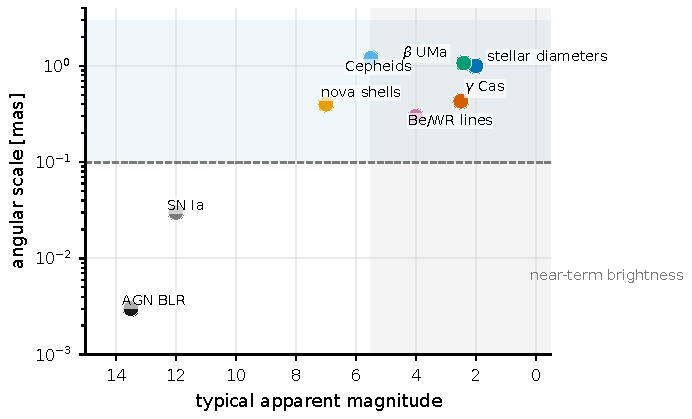
\includegraphics[width=0.88\linewidth]{figures/generated/chapter_19/ch19_science_case_feasibility.pdf}
\caption{第一代候选目标在"亮度--角尺度"平面上的位置。亮星角直径、\(\beta\) UMa、\(\gamma\) Cas 以及 Be/WR 谱线区同时满足"够亮"和"能被百米级基线解析"，落在最舒服的区域；Type Ia、AGN 宽线区和暗物质小尺度透镜科学价值很高，却被亮度、事件率或角尺度推向长期项目。这张图就是式 \eqref{eq:e25-priority-score} 里三把尺子的可视化。}
\label{fig:e25-case-plane}
\end{figure}

有了这套排序，本章后面的顺序其实已经隐含其中：先做落在图 \ref{fig:e25-case-plane} 右上"舒服区"的目标，再一步步往科学价值更高、但风险也更大的方向推进。

\section{恒星角直径与有效温度：第一代最成熟的产品}
\label{sec:e25-diameter}

为什么第一件事是量恒星的\textbf{角直径}（angular diameter）？因为它同时满足前面三把尺子，而且产出直接、可复现、能反复当验收标准。观测量非常干净：在一系列基线 \(B\) 和波长 \(\lambda\) 上测平方可见度 \(|V|^2(B,\lambda)\)，模型从最简单的\textbf{均匀圆盘}（uniform disk）开始，再用\textbf{边缘昏暗}（limb darkening，恒星盘边缘比中心暗）廓线或完整大气模型去修正。

角直径最漂亮的用处，是它能直接钉住恒星的\textbf{有效温度}（effective temperature）。这里的逻辑链一步都不能跳，我们把它铺开。一颗半径 \(R\)、有效温度 \(T_{\rm eff}\) 的恒星，其光度由 Stefan--Boltzmann 定律给出 \(L=4\pi R^2\sigma_{\rm SB}T_{\rm eff}^4\)。这些光子跑到距离 \(D\) 的地球，摊在一个半径为 \(D\) 的球面上，于是我们收到的\textbf{总辐射流量}（bolometric flux）是
\[
  F_{\rm bol}=\frac{L}{4\pi D^2}
  =\frac{R^2}{D^2}\,\sigma_{\rm SB}T_{\rm eff}^4
  =\left(\frac{R}{D}\right)^2\sigma_{\rm SB}T_{\rm eff}^4 .
\]
注意 \(R/D\) 正是恒星的\textbf{角半径}，而角直径 \(\theta_{\rm LD}=2R/D\)，所以 \(R/D=\theta_{\rm LD}/2\)，\((R/D)^2=\theta_{\rm LD}^2/4\)。代回去就得到本节的核心式：
\begin{equation}
  F_{\rm bol}
  =
  \frac{\theta_{\rm LD}^2}{4}
  \sigma_{\rm SB}T_{\rm eff}^4,
  \qquad
  T_{\rm eff}
  =
  \left(
  \frac{4F_{\rm bol}}
  {\sigma_{\rm SB}\theta_{\rm LD}^2}
  \right)^{1/4}.
  \label{eq:e25-teff}
\end{equation}
\begin{formulaexplain}
\(F_{\rm bol}\) 是地球处收到的总辐射流量，\(\theta_{\rm LD}\) 是边缘昏暗角直径，\(\sigma_{\rm SB}\) 是 Stefan--Boltzmann 常数，\(T_{\rm eff}\) 是有效温度。一句话：角直径一旦测准，就能把"流量"直接换算成恒星的"温度尺"。
\end{formulaexplain}
逐个交代单位与量纲：\(F_{\rm bol}\) 单位 \(\mathrm{erg\,s^{-1}\,cm^{-2}}\)，从多波段测光积分得到；\(\theta_{\rm LD}\) 单位 rad（毫角秒 mas 是常用的实用单位，\(1\,\mathrm{mas}=4.85\times10^{-9}\,\mathrm{rad}\)）；\(\sigma_{\rm SB}=5.67\times10^{-5}\,\mathrm{erg\,s^{-1}\,cm^{-2}\,K^{-4}}\)；\(T_{\rm eff}\) 单位 K。这条式子妙在它\textbf{不依赖距离}：\(F_{\rm bol}\) 和 \(\theta_{\rm LD}\) 都是直接可观测的，中间那个 \(D\) 在推导里已经消掉了。

角直径的误差怎样传到温度上？把 \(T_{\rm eff}\) 对 \(\theta_{\rm LD}\) 取对数微分。因为 \(T_{\rm eff}\propto\theta_{\rm LD}^{-1/2}\)（把 \(F_{\rm bol}\) 视为独立测量），有
\[
  \ln T_{\rm eff}=\text{常数}-\tfrac12\ln\theta_{\rm LD}
  \;\Longrightarrow\;
  \frac{\delta T_{\rm eff}}{T_{\rm eff}}=-\frac12\frac{\delta\theta_{\rm LD}}{\theta_{\rm LD}} .
\]
所以角直径 \(4\%\) 的误差，只由这一路传播到温度，就是 \(2\%\)。这个"减半"的关系解释了为什么亮星角直径值得反复测：它不是一次性的仪器炫技，而是会流进 \(T_{\rm eff}\)、恒星半径、年龄、自转模型和标准星尺度的\textbf{基石数据} \citep{1967MNRAS.137..393H,1977MNRAS.180..177B,2003RPPh...66..789M}。

这条路线已经从历史走进了现代。上世纪 Narrabri 强度干涉仪用 Hanbury Brown 和 Twiss 的方法量过一批亮星直径 \citep{1956Natur.178.1046H,1974MNRAS.167..121H}；今天 VERITAS 的强度干涉系统（VERITAS-SII）把它推进到亚毫角秒精度，对 \(\beta\) CMa 和 \(\epsilon\) Ori 给出直径，且用远少于当年的观测时间就做到优于 \(5\%\)；后续对 \(\beta\) UMa 在 416 nm 得到边缘昏暗角直径 \(\theta_{\rm LD}=1.07\pm0.04_{\rm stat}\pm0.05_{\rm sys}\,\mathrm{mas}\)，并与 CHARA 近红外、Keck 中红外结果互相校验。MAGIC 的升级系统（MAGIC-SII）更是一口气报告了 22 个恒星直径，其中 13 个此前没有可比测量——强度干涉已经从"单次演示"变成"成批出数据" \citep{2020NatAs...4.1164A,2024ApJ...966...28A,2024MNRAS.529.4387A}。这里要提醒的一点是：这些结果用的是\textbf{二阶}相干（第 \ref{chap:e08}、\ref{chap:e10} 章），它对大气宁静度和光路相位不敏感，这正是它在窄带、超长基线上仍能工作的原因。

\textbf{要什么、答什么？}这一案例需要的阵列很朴素：几对现成 IACT 望远镜、百米级基线、窄带滤光、GHz 级电子带宽、几小时到几夜的积分；精度目标是把直径做到 \(3\text{--}5\%\)、多夜可复现。它回答的是恒星物理里最基础的问题——\textbf{这颗星到底多大、多热}，进而校准整条恒星参数与距离尺度。

\section{快速自转：从"多大"升级到"什么形状"}
\label{sec:e25-rotation}

量到直径只是第一步。很多热星转得极快，快到离心力把赤道甩得鼓出来，光球变成一个扁椭球；而且按 von Zeipel 定理，鼓出去的赤道引力小、温度低、更暗，两极则又亮又热——这就是\textbf{重力昏暗}（gravity darkening）。要看见这种结构，均匀圆盘模型就不够了：它只有一个参数 \(\theta\)，而一个扁椭球至少需要三个参数——短轴角直径 \(\theta_{\rm min}\)、\textbf{轴比}（axial ratio）\(r=\theta_{\rm maj}/\theta_{\rm min}\)、以及位置角 \(\varphi_\star\)。

怎样把这个扁球写成可拟合的可见度曲线？先回忆第 \ref{chap:e11} 章的已知结果：一个角直径为 \(\theta\) 的均匀圆盘，其一阶可见度模长是 Airy 形式 \(|V|=|2J_1(x)/x|\)，其中 \(x=\pi B\theta/\lambda\) 是无量纲空间频率，\(J_1\) 是一阶 Bessel 函数（圆孔径衍射的标准结果，第一个零点在辐角 \(3.83\)）。椭球的诀窍在于：沿不同方向投影，看到的"有效直径"不同——沿短轴看是 \(\theta_{\rm min}\)，沿长轴看是 \(r\theta_{\rm min}\)。把这个方向依赖装进 \(x\)，就得到
\begin{equation}
  x_{\rm ell}
  =
  \frac{\pi B_p\theta_{\rm min}}{\lambda}
  \left[
  \cos^2\psi
  +
  r^2\sin^2\psi
  \right]^{1/2},
  \qquad
  |V_{\rm ell}|^2
  =
  \left[\frac{2J_1(x_{\rm ell})}{x_{\rm ell}}\right]^2 .
  \label{eq:e25-elliptical-visibility}
\end{equation}
\begin{formulaexplain}
\(x_{\rm ell}\) 是扁椭球在当前投影基线上的无量纲空间频率，\(B_p\) 是投影基线长度，\(\psi\) 是投影基线相对短轴的方向角，\(r\) 是轴比。方括号里的因子把"看的方向"折进了有效直径：沿短轴（\(\psi=0\)）它退回 \(\theta_{\rm min}\)，沿长轴（\(\psi=90^\circ\)）它变成 \(r\theta_{\rm min}\)。
\end{formulaexplain}
把方括号验一眼就懂它的几何：当 \(\psi=0\)（基线正对短轴），\(\cos^2\psi=1,\sin^2\psi=0\)，\(x_{\rm ell}=\pi B_p\theta_{\rm min}/\lambda\)，看到的是短轴；当 \(\psi=90^\circ\)，\(x_{\rm ell}=\pi B_p(r\theta_{\rm min})/\lambda\)，看到的是长轴。参数落地：热星轴比典型在 \(r\simeq1.1\text{--}1.5\)，短轴角直径常小于 \(1\,\mathrm{mas}\)。这里有个关键的\textbf{观测设计}教训：要同时钉住 \(r\) 和 \(\varphi_\star\)，你必须在\textbf{多个位置角}上都拿到 \(|V|^2\)——单方向的基线覆盖会让 \(r\) 和 \(\varphi_\star\) 严重退化，因为一条曲线可以由"更扁但转个角度"和"没那么扁"共同拟合。这正是第 \ref{chap:e11} 章 uv 覆盖那套语言在具体目标上的兑现。

现实里这已经做出来了。VERITAS 对经典快速自转星 \(\gamma\) Cas 的观测给出短轴角直径约 \(0.43\pm0.02_{\rm stat}\pm0.02_{\rm sys}\,\mathrm{mas}\)、轴比约 \(1.28\pm0.04\pm0.02\)、自转轴位置角约 \(116^\circ\)，并用 Roche--von Zeipel 模型推断它已接近\textbf{临界自转}（breakup rotation，赤道离心力接近平衡引力）\citep{2025ApJ...995..191A}。这意味着第一代强度干涉已经能从"这颗星多大"推进到"这颗星是什么形状、两极和赤道差多少温度"。

\textbf{要什么、答什么？}这一案例需要在同一目标上覆盖\textbf{两个以上明显不同的位置角}，其余要求与角直径相同；精度目标是能在统计上区分圆盘模型与椭圆模型。它回答的是恒星结构与演化里的一个深问题——\textbf{自转如何改变恒星的形状、温度分布乃至寿命}。

\section{双星、Be 星盘与 Wolf--Rayet 风：用基线把它们分开}
\label{sec:e25-binary}

强度干涉不止能测"一个源有多大"，也能把"其实是两个源"识破。\textbf{密近双星}（close binary）的好处是它的信号有极高的辨识度。设两个都未被解析的点源，角分离向量为 \(\bm s\)，\textbf{流量比}（flux ratio）\(f=F_2/F_1\)。它们的合成相干函数是各自复振幅按流量加权的叠加，归一化后为 \((1+f\,e^{-2\pi i\,\bm u\cdot\bm s})/(1+f)\)，其中 \(\bm u=\bm B_\perp/\lambda\) 是空间频率。平方可见度就是它的模平方，我们把这一步展开，一格都不跳：
\[
  |V_{\rm binary}|^2
  =\frac{|1+f e^{-i\phi}|^2}{(1+f)^2},
  \qquad \phi\equiv 2\pi\,\bm u\cdot\bm s .
\]
利用 \(|1+f e^{-i\phi}|^2=(1+f\cos\phi)^2+(f\sin\phi)^2=1+2f\cos\phi+f^2\cos^2\phi+f^2\sin^2\phi=1+f^2+2f\cos\phi\)（这里只用了 \(\cos^2+\sin^2=1\)），得到
\begin{equation}
  |V_{\rm binary}|^2
  =
  \frac{1+f^2+2f\cos(2\pi\,\bm u\cdot\bm s)}
  {(1+f)^2}.
  \label{eq:e25-binary-visibility}
\end{equation}
\begin{formulaexplain}
\(\bm u=\bm B_\perp/\lambda\) 是空间频率，\(\bm s\) 是双星角分离向量，\(f\) 是流量比。指数里的相位随基线变化，使 \(|V|^2\) 沿基线上下\textbf{振荡}——正是这条振荡曲线让强度干涉能约束双星的分离与方向。
\end{formulaexplain}
读这条式子的关键是那个余弦项的\textbf{振幅} \(2f/(1+f)^2\)。当 \(f=1\)（等亮双星），\(|V|^2\) 会从 \(1\)（当 \(\cos=+1\)）一路振荡到 \(0\)（当 \(\cos=-1\)），信号又深又好认；当 \(f=0.1\)（暗伴星只有主星十分之一亮），余弦项的半振幅只剩 \(2(0.1)/(1.1)^2\simeq0.17\)，而 \(|V|^2\) 是围绕均值 \((1+f^2)/(1+f)^2=1.01/1.21\simeq0.83\) 上下摆动这个半振幅，也就是从谷值 \((1-f)^2/(1+f)^2=(0.9/1.1)^2\simeq0.67\) 起伏到峰值 \(1.0\)，调制深度只有约 \(0.33\)，对信噪比和校准的要求陡然提高。振荡的\textbf{周期}则由分离 \(\bm s\) 定：分离越大，\(|V|^2\) 随基线振荡越快。所以双星项目最适合那些\textbf{已有光谱轨道或食双星先验}的系统——每夜只需拿到少数几个基线点，就能被已知轨道模型串起来；即便某夜失败，也能给出分离或亮度比的上限，不至于颗粒无收 \citep{1974MNRAS.167..121H,2012MNRAS.419..172N,2014MNRAS.437..798M,2022MNRAS.512.1722K}。

\begin{figure}[tbp]
\centering
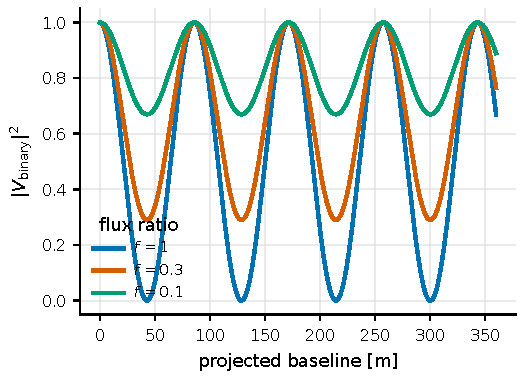
\includegraphics[width=0.82\linewidth]{figures/generated/chapter_19/ch19_binary_visibility.pdf}
\caption{一对 \(1\,\mathrm{mas}\) 双星在 416 nm 下的平方可见度振荡。等亮双星（\(f=1\)）给出从 1 到 0 的深振荡；流量比降到 \(0.3\)、\(0.1\) 后，按式 \eqref{eq:e25-binary-visibility} 的振幅 \(2f/(1+f)^2\) 迅速变浅。双星项目因此格外依赖多位置角的基线覆盖和已知轨道先验，否则亮度比、分离和位置角会互相退化。}
\label{fig:e25-binary-visibility}
\end{figure}

再往前一步，是把"空间分辨"和"谱线选择"结合起来，去解剖\textbf{Be 星盘}（Be decretion disk，快速自转 B 型星抛出的赤道气盘）和\textbf{Wolf--Rayet 风}（大质量恒星的高速星风）。这些源的连续谱主要来自光球，而 \(\mathrm{H}\alpha\)、He、Fe 等发射线却来自更大、更扩展的盘或风碰撞区。麻烦在于，一个滤光片里往往\textbf{谱线和连续谱混在一起}，测到的可见度是两者按通量加权的平均：
\begin{equation}
  V_{\rm obs}
  =
  \frac{
  F_{\rm c}V_{\rm c}
  +
  F_{\rm line}V_{\rm line}
  }{
  F_{\rm c}+F_{\rm line}
  } .
  \label{eq:e25-line-continuum}
\end{equation}
\begin{formulaexplain}
\(V_{\rm c},V_{\rm line}\) 分别是连续谱区与谱线区的可见度，\(F_{\rm c},F_{\rm line}\) 是对应通量。你测到的 \(V_{\rm obs}\) 是二者的通量加权平均，所以谱线几何必须先从连续谱里"减"出来，才能单独解释。
\end{formulaexplain}
其中 \(F_{\rm line}/F_{\rm c}\) 可从同时光谱或"窄带减连续谱"的双滤光片估计。物理判读很直观：如果谱线区比光球\textbf{大}（如展开的盘），那么长基线上的 \(V_{\rm line}\) 会比连续谱掉得更快，混合后的 \(V_{\rm obs}\) 在长基线端被谱线拖低；反过来，如果谱线来自一个很小的高亮斑，长基线上它反而保留信号。历史上 Narrabri 对 Wolf--Rayet 双星 \(\gamma^2\) Velorum 就已经展示了发射线区和连续谱区可以有\textbf{不同的角尺度} \citep{1970MNRAS.148..103H,2010SPIE.7734E..0AD,2012NewAR..56..143D,2025ApJ...995..191A}。现代多基线阵列可以把这一思想推广到 Be 星盘的几何、快速自转热星的谱线轮廓，以及相互作用双星的风碰撞区。

\textbf{要什么、答什么？}这一案例需要窄带滤光或同时光谱来分离谱线与连续谱、可验证的连续谱扣除、以及足够的谱线通量；它回答的是\textbf{恒星如何抛出物质、盘和风是什么几何形状}这类难以用别的手段直接成像的问题。

\section{膨胀的瞬变：新星现在能做，Type Ia 是长期目标}
\label{sec:e25-transient}

现在把镜头转向会"长大"的源。新星、超新星这类爆发抛出一团膨胀外壳，它的几何账本极其简单：若外壳以速度 \(v_{\rm exp}\) 近似自由膨胀，那么爆发后时间 \(t-t_0\) 时，它张开的角直径是"走过的线半径的两倍除以距离"：
\begin{equation}
  \theta(t)
  \simeq
  \frac{2v_{\rm exp}(t-t_0)}{D},
  \qquad
  D
  \simeq
  \frac{2v_{\rm exp}(t-t_0)}{\theta}.
  \label{eq:e25-expansion}
\end{equation}
\begin{formulaexplain}
\(\theta(t)\) 是膨胀外壳的角直径，\(v_{\rm exp}\) 是膨胀速度，\(t_0\) 是爆发时刻，\(D\) 是距离。左式预言"外壳有多大"，右式反解出"离我们多远"——这就是不依赖标准烛光的\textbf{膨胀视差}（expansion parallax）。
\end{formulaexplain}
逐项交代：\(v_{\rm exp}\) 来自谱线的多普勒速度（第 \ref{chap:e20} 章讲过怎样从波长移动读速度），单位 \(\mathrm{cm\,s^{-1}}\)；\(t-t_0\) 是爆发后时间，单位 s；\(D\) 是距离，单位 cm。它的物理前提是一句大白话：\(v_{\rm exp}\) 和 \(\theta\) 必须对应\textbf{同一层物质}，否则右式的距离会系统性偏差（第 \ref{chap:e20} 章详细分析过这个陷阱）。

把两组真实数字代进去，第一代能做什么、不能做什么立刻见分晓。\textbf{银河系新星}：取 \(D=2\,\mathrm{kpc}=6.17\times10^{21}\,\mathrm{cm}\)、\(v_{\rm exp}=10^8\,\mathrm{cm\,s^{-1}}\)、\(t-t_0=10\,\mathrm{d}=8.64\times10^5\,\mathrm{s}\)。线半径 \(v_{\rm exp}(t-t_0)=8.64\times10^{13}\,\mathrm{cm}\)，角直径 \(\theta=\dfrac{2\times8.64\times10^{13}}{6.17\times10^{21}}=2.80\times10^{-8}\,\mathrm{rad}\)。用 \(1\,\mathrm{rad}=2.063\times10^8\,\mathrm{mas}\) 换算，\(\theta\approx5.8\,\mathrm{mas}\)——十天后就到了几毫角秒，用百米以下基线即可解析。\textbf{Type Ia 超新星}：取 \(D=10\,\mathrm{Mpc}=3.09\times10^{25}\,\mathrm{cm}\)、\(v_{\rm exp}=10^9\,\mathrm{cm\,s^{-1}}\)、\(t-t_0=20\,\mathrm{d}=1.73\times10^6\,\mathrm{s}\)。线半径 \(1.73\times10^{15}\,\mathrm{cm}\)，\(\theta=\dfrac{2\times1.73\times10^{15}}{3.09\times10^{25}}=1.12\times10^{-10}\,\mathrm{rad}\approx0.023\,\mathrm{mas}\)——即便速度快十倍，二十天后也只有几十微角秒，需要\textbf{数公里}级光学基线才能碰到。

\begin{figure}[tbp]
\centering
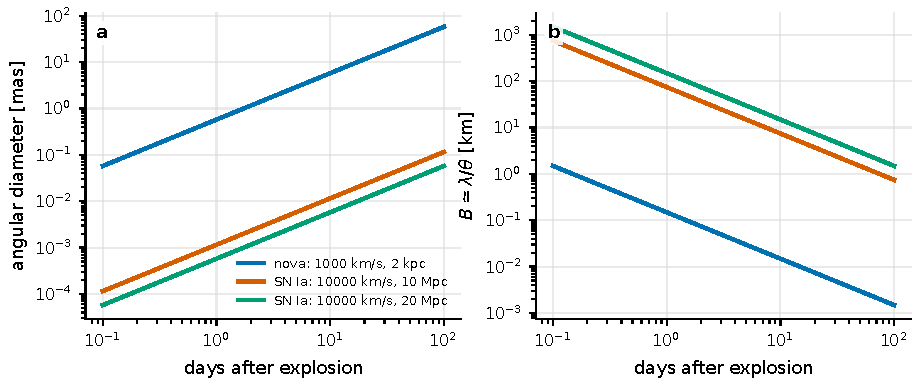
\includegraphics[width=0.94\linewidth]{figures/generated/chapter_19/ch19_transient_expansion.pdf}
\caption{膨胀瞬变的角直径与所需基线。银河系新星在几天到几十天内进入毫角秒量级，适合第一代拿来做"触发--调度--成像"的整套演练；\(10\text{--}20\,\mathrm{Mpc}\) 的 Type Ia 即使在峰值附近也只有几十微角秒，需要公里级基线和 \(m\lesssim12\) 的近邻事件。曲线正是式 \eqref{eq:e25-expansion} 在不同 \(v_{\rm exp}\)、\(D\) 下的走向。}
\label{fig:e25-transient-expansion}
\end{figure}

所以第一代的分工很清楚：\textbf{银河系新星}是现实目标，它角尺度够大、又足够亮，最适合用来把触发（trigger）、滤光、背景扣除、模型拟合的整条流水线跑通，主要困难来自亮度快速演化、外壳非球对称和尘埃遮挡。\textbf{Type Ia 几何距离}则是高回报的长期目标：Kim 等的可行性研究把 \(m\lesssim12\)（对应 \(z\sim0.004\) 的局部体积，全天约每年一个）作为可预见下一代的亮度范围，并用辐射转移模型算出不同波长的表面亮度与 \(|V|^2\)，指出\textbf{光谱分辨}可以提供多波长层析，让测量不再局限于一个均匀圆盘半径 \citep{2025PhRvD.111h3047K,1997A&A...320..799F,2004A&A...415..531S}。换句话说，Type Ia 距离标尺应当排进二代或专用阵列的目标，而不是第一代的验收项。

\textbf{要什么、答什么？}新星案例需要\textbf{快速触发}（几小时内响应）加上同时的谱线速度，把 \(\theta(t)\) 和 \(v_{\rm exp}\) 配对；它回答的是"这次爆发离我们多远、外壳是不是球对称"，并为将来用膨胀视差独立校准宇宙距离阶梯做技术铺垫。

\section{Crab 与自然激光：用光子统计检验"非热"}
\label{sec:e25-statistics}

前面几节都在用\textbf{可见度}（二阶相干的空间信息）。本节换一副眼镜，用\textbf{时间统计}——这正是事件表（第 \ref{chap:e13} 章）和 \(g^{(2)}\)（第 \ref{chap:e08} 章）大显身手的地方。

先说 \textbf{Crab 脉冲星}。它并不是空间强度干涉的好目标（它是个点源），但它是事件表科学的绝佳对象：亮、周期稳、有精确星历（ephemeris），光学主脉冲和 interpulse 能定义清晰的\textbf{相位窗}（phase window）。把每个光子放进正确相位窗的前提，是时间戳足够准。相位误差与时间误差的换算简单到一行：
\begin{equation}
  \Delta\phi
  =
  \frac{\Delta t}{P_{\rm spin}}.
  \label{eq:e25-pulse-phase}
\end{equation}
\begin{formulaexplain}
\(\Delta t\) 是光子时间戳误差，\(P_{\rm spin}\) 是脉冲星自转周期，\(\Delta\phi\) 是折算出的相位误差（无量纲，\(0\text{--}1\) 对应一整周）。时间越准，光子越能被放进它真正所属的脉冲相位窗。
\end{formulaexplain}
代数量级：Crab 的 \(P_{\rm spin}\simeq33\,\mathrm{ms}\)，一个 \(1\,\mu\mathrm{s}\) 的时间误差只对应 \(\Delta\phi\simeq10^{-6}/(33\times10^{-3})\approx3\times10^{-5}\)——极其宽裕，微秒级同步足矣。但同样一条式子告诉你，毫秒脉冲星（\(P\sim\mathrm{ms}\)）要保留同样窄的相位结构，就得把 \(\Delta t\) 压到纳秒量级。有了相位窗，就能做过去平均光变曲线做不了的事：相位分辨的 \(g^{(2)}\)、颜色相关、以及和射电\textbf{巨脉冲}（giant pulse）的条件叠加。AquEYE/Iqueye 这类仪器已经能把光子打上皮秒到纳秒的时间标签保存下来；观测上，Crab 巨射电脉冲所在周期的光学发射有增强，ARCONS 还看到早到的巨脉冲对应更强的光学增强 \citep{2009JMOp...56..261B,2009A&A...508..531N,2015SPIE.9504E..0CZ,2003Sci...301..493S,2013ApJ...779L..12S}。第一代量子天文学要做的，就是把这些结果从"平均光变"升级成"事件表统计 + 偏振/颜色分窗"。

\begin{figure}[tbp]
\centering
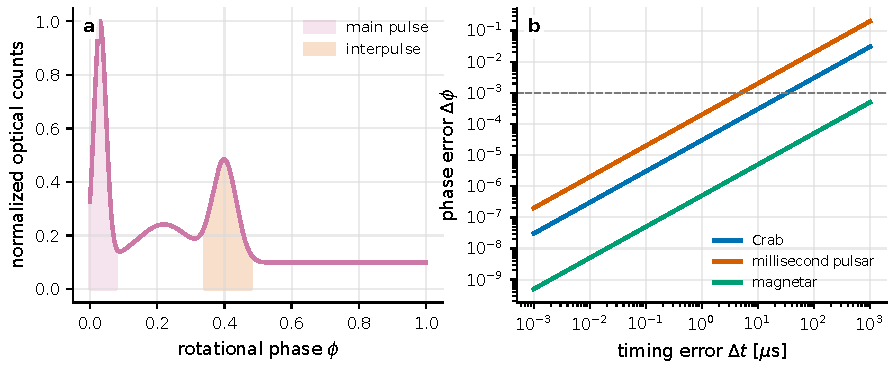
\includegraphics[width=0.94\linewidth]{figures/generated/chapter_19/ch19_crab_phase_windows.pdf}
\caption{Crab 型光学脉冲的相位窗与时间误差。左图示意主脉冲、bridge 和 interpulse 三个事件选择窗；右图把时间误差按式 \eqref{eq:e25-pulse-phase} 换成相位误差。对 Crab，微秒级时间已经绰绰有余；对毫秒脉冲星，则要 ns--\(\mu\mathrm{s}\) 级同步才能保住窄相位结构。}
\label{fig:e25-crab-phase}
\end{figure}

再说\textbf{自然激光}（natural / astrophysical laser）候选。这类目标要检验的是一个很纯粹的量子问题：\textbf{这条亮谱线的光子统计，到底是热的还是相干的？}但要小心一个陷阱——"看到一条亮谱线"本身\textbf{不足以}断言是激光，因为多个互不相干的热模式叠加也能让聚束（bunching）峰被平均掉。定量地说，对 \(M\) 个互不相干的热模式，
\begin{equation}
  g^{(2)}(0)-1
  =
  \frac{1}{M},
  \label{eq:e25-mode-bunching}
\end{equation}
\begin{formulaexplain}
\(M\) 是探测里叠加的互不相干热模式数，\(g^{(2)}(0)\) 是零延迟二阶相干。单模热光有 \(g^{(2)}(0)=2\)（聚束），但 \(M\) 越大，聚束峰被越平均掉，\(g^{(2)}(0)\to1\)。所以 \(g^{(2)}(0)\) 接近 1 并不必然说明光是理想激光。
\end{formulaexplain}
对照记住第 \ref{chap:e08} 章两个极端：单模热态 \(g^{(2)}(0)=2\)、理想相干态（coherent state）\(g^{(2)}(0)=1\)。式 \eqref{eq:e25-mode-bunching} 说的是"多模热光会伪装成相干光"，所以做这类检验必须配一个\textbf{零假设检验}（null test）——把模式数、仪器时间响应、连续谱背景都算清楚，才能判断 \(g^{(2)}(0)\) 偏离 1 或接近 1 意味着什么。另一个可用的把手是谱线宽度：若线宽为 \(\Delta\nu\)，相干时间约 \(\tau_c\sim1/(\pi\Delta\nu)\)（第 \ref{chap:e02} 章带宽--相干时间关系的具体化）。举例，若一条自然激光线窄到 \(\Delta\nu\sim1\,\mathrm{GHz}\)，则 \(\tau_c\sim1/(\pi\times10^9)\approx3\times10^{-10}\,\mathrm{s}=0.3\,\mathrm{ns}\)；线越窄、相干时间越长，在给定探测器时间分辨率下越容易保留可解析的相关\textbf{对比度}（contrast）。真实候选里，Eta Carinae 的 Weigelt blobs 中 Fe II 线被 \(\mathrm{Ly}\alpha\) 泵浦（pumping），Johansson 与 Letokhov 讨论过 \(0.9\text{--}1.0\,\mu\mathrm{m}\) 及近红外的 Fe II 激光线；线宽测量加光子相关谱学（photon-correlation spectroscopy）可以给出直接证据 \citep{2004A&A...428..497J,2005NewA...10..361J,2008AIPC..984..216D}。

\begin{figure}[tbp]
\centering
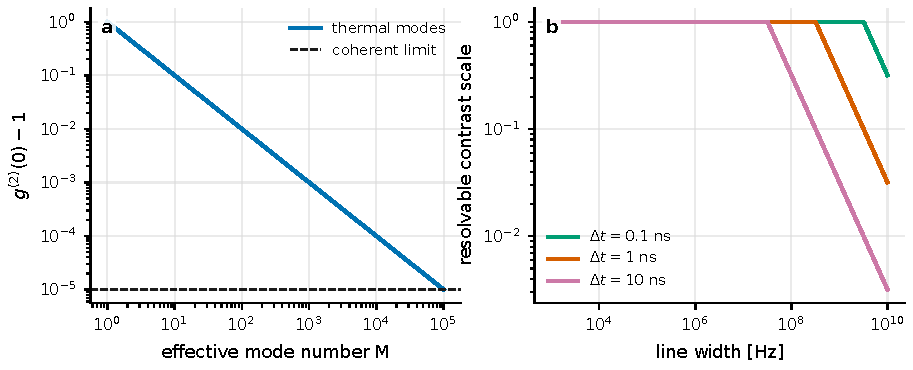
\includegraphics[width=0.94\linewidth]{figures/generated/chapter_19/ch19_natural_laser_statistics.pdf}
\caption{自然激光候选的两个统计判据。左图显示热光模式数 \(M\) 增大会把聚束峰按式 \eqref{eq:e25-mode-bunching} 压低，逼近相干极限 \(g^{(2)}(0)-1=0\)；右图显示线宽越窄、相干时间越长，在给定时间分辨率下越容易保留可解析对比度。二者说明：判断"是否激光"需要联合光子统计与线宽，并做严格的零假设检验。}
\label{fig:e25-natural-laser}
\end{figure}

\textbf{要什么、答什么？}这两类案例更依赖\textbf{事件表质量}——绝对时间同步、精确星历、可验证的背景扣除、以及能分离谱线与连续谱的窄带筛选；它们回答的是"这束光的量子统计是什么性质"，把辐射机制（第 \ref{chap:e16} 章）从光谱层面推到光子统计层面。

\section{把清单排成路线：顺序随仪器成熟而变}
\label{sec:e25-roadmap}

把上面所有案例摆进同一张矩阵，第一代的推进顺序主要由\textbf{技术成熟度}和\textbf{系统风险}决定，而不是纯凭科学价值。图 \ref{fig:e25-priority} 就是这张矩阵：横轴是技术成熟度、纵轴是科学回报、点越大表示系统与触发风险越高。

\begin{figure}[!htbp]
\centering
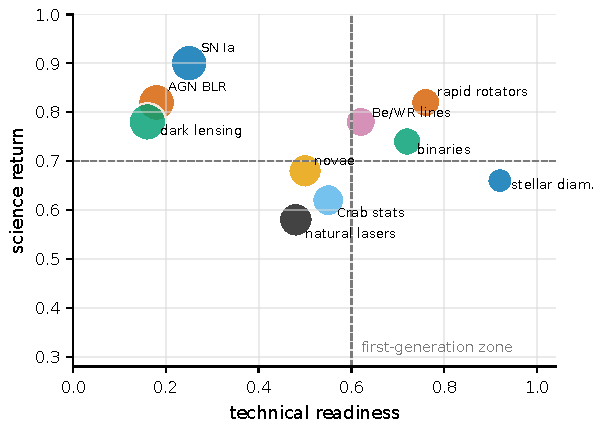
\includegraphics[width=0.78\linewidth]{figures/generated/chapter_19/ch19_priority_matrix.pdf}
\caption{第一代科学案例矩阵。横轴技术成熟度、纵轴科学回报，点越大代表系统误差与触发风险越高。右上方且点较小的目标最适合作为第一代验收；左上方目标（Type Ia、AGN 宽线区、暗物质小尺度透镜）科学价值高，却需要专用阵列或更成熟的量子资源，属长期目标。}
\label{fig:e25-priority}
\end{figure}

读法是这样的：\textbf{右上且点小}的目标（亮热星角直径、已知直径的参考星、\(\beta\) UMa 类 A 型星、MAGIC/VERITAS 可重复目标）风险低、能复现，天然是第一批验收项目；在同一套能力上继续增加科学信息的，是 \(\gamma\) Cas 类快速自转、Be/WR 谱线区、密近双星和新星早期膨胀；更依赖事件表质量与时间/光谱筛选的，是 Crab 相位分辨统计和自然激光候选线；而左上方那些高价值目标——Type Ia 几何距离、AGN 宽线区、暗物质小尺度透镜、量子网络辅助成像（第 \ref{chap:e24} 章）——则应稳稳放在长期目标里。

下面这张表把七类案例的第一观测量、典型数量级和"能不能算第一代"的判据并排列出，便于对照。它其实就是把式 \eqref{eq:e25-priority-score} 那套排序落成一份可执行清单：

\begin{longtable}{p{0.17\linewidth}p{0.22\linewidth}p{0.23\linewidth}p{0.20\linewidth}}
\toprule
案例 & 第一观测量 & 典型数量级 & 第一代判据 \\
\midrule
亮星角直径 & \(|V|^2(B)\) & \(m_V<5\)，\(\theta=0.5\text{--}2\,\mathrm{mas}\) & 多夜重复到 \(3\text{--}5\%\) 直径精度。 \\
快速自转 & 多位置角 \(|V|^2\) & 轴比 \(1.1\text{--}1.5\)，\(\theta<1\,\mathrm{mas}\) & 能区分圆盘与椭圆模型。 \\
双星 & \(|V|^2\) 振荡 & 分离 \(0.2\text{--}5\,\mathrm{mas}\)，\(f>0.1\) & 已有轨道先验，覆盖两个以上位置角。 \\
Be/WR 谱线 & 谱线/连续谱 \(|V|^2\) & \(\mathrm{H}\alpha\)、He、Fe 线 & 线通量足够，连续谱扣除可验证。 \\
新星 & \(\theta(t)\) & 几天后 mas 量级 & 触发快，能与谱线速度合并。 \\
Crab 统计 & 相位窗 \(g^{(2)}\)、颜色相关 & \(P=33\,\mathrm{ms}\) & 星历、背景星云与绝对时间闭合。 \\
自然激光 & \(g^{(2)}\)、线宽、偏振 & \(\Delta\nu\) 可窄到高相干时间 & 谱线可与连续谱分离，有零假设检验。 \\
Type Ia & \(|V|^2(\lambda,t)\) & \(m<12\)，几十 \(\mu\mathrm{as}\) & 公里级阵列与快速触发成熟后再做。 \\
\bottomrule
\end{longtable}

排序会随仪器状态动态改变，这一点很重要。系统刚完成时间同步和零基线相关标定时，亮星角直径和参考星复现最有价值；当六条以上基线能稳定运行、uv 覆盖变好，快速自转和双星进入主清单；当窄带滤光和高数据吞吐可靠，自然激光和谱线盘才有现实空间；只有当阵列扩到公里级、并能每年快速响应 \(m\lesssim12\) 的近邻瞬变时，Type Ia 几何距离才会升为第一线目标 \citep{2017MNRAS.472.4126G,2022MNRAS.512.1722K,2024MNRAS.529.4387A,2024ApJ...966...28A,2025ApJ...995..191A,2025PhRvD.111h3047K}。所有这些取舍，最终都要回到第 \ref{chap:e15} 章的误差预算里去逐条核账——这也是下一部分教学与计算实验（第 \ref{chap:e26} 章）要带你亲手跑一遍的东西。

\section*{本章要点}
\addcontentsline{toc}{section}{本章要点}

\begin{itemize}
  \item \textbf{先排序，再观测。} 用亮度、角尺度、外部先验三把尺子给案例分诊，写成排序式 \eqref{eq:e25-priority-score}：科学回报、技术成熟度、先验提分，系统与触发风险减分。第一代要挑"右上舒服区"的目标，别被漂亮题目牵着走。
  \item \textbf{角直径是第一代最成熟的产品。} 它经均匀圆盘/边缘昏暗模型直接进入有效温度式 \eqref{eq:e25-teff}，且 \(T_{\rm eff}\propto\theta^{-1/2}\) 让 \(4\%\) 的直径误差只传成 \(2\%\) 的温度误差。VERITAS、MAGIC 已在成批出数据。
  \item \textbf{从"多大"到"什么形状"。} 快速自转星要用椭圆可见度式 \eqref{eq:e25-elliptical-visibility}，且必须覆盖多个位置角才能钉住轴比与位置角；\(\gamma\) Cas 已被测出接近临界自转。
  \item \textbf{双星与谱线盘靠基线分辨。} 双星的 \(|V|^2\) 按式 \eqref{eq:e25-binary-visibility} 振荡，振幅 \(2f/(1+f)^2\) 随流量比迅速变小；谱线与连续谱按通量加权混合（式 \eqref{eq:e25-line-continuum}），必须先分离再解释。
  \item \textbf{膨胀瞬变分远近。} 角膨胀式 \eqref{eq:e25-expansion} 给出膨胀视差：银河系新星几天就到 mas，是现实目标；\(10\,\mathrm{Mpc}\) 的 Type Ia 只有几十 \(\mu\mathrm{as}\)，是需要公里级阵列的长期目标。
  \item \textbf{光子统计检验"非热"。} Crab 用相位窗式 \eqref{eq:e25-pulse-phase} 做相位分辨 \(g^{(2)}\)；自然激光要用多模关系式 \eqref{eq:e25-mode-bunching} 加线宽做零假设检验，因为多模热光会伪装成相干光。
  \item \textbf{顺序随仪器成熟而变。} 从零基线标定、到多基线、到窄带高吞吐、再到公里级快响应，路线图是动态的，最终都要回到第 \ref{chap:e15} 章误差预算逐条核账。
\end{itemize}

\medskip
\noindent\textbf{想一想}
\begin{itemize}
  \item 若某亮星角直径测到 \(3\%\) 精度，且总辐射流量 \(F_{\rm bol}\) 也有 \(3\%\) 的独立误差，用式 \eqref{eq:e25-teff} 估一下有效温度 \(T_{\rm eff}\) 的相对误差大约多少？（提示：先分别求 \(T\) 对 \(\theta\) 和对 \(F\) 的对数灵敏度，再按独立误差平方相加。）
  \item 一对流量比 \(f=0.05\) 的双星，用式 \eqref{eq:e25-binary-visibility} 算它 \(|V|^2\) 振荡的余弦振幅是多少？要在 \(1\) 小时内把它测出来，对光子对数和系统校准提出了什么要求（回顾第 \ref{chap:e15} 章）？
  \item 为什么"看到一条又亮又窄的谱线"还不足以断定它是自然激光？式 \eqref{eq:e25-mode-bunching} 里的 \(M\) 在这个判断里扮演什么角色，你会设计一个怎样的零假设检验来排除"多模热光伪装"？
\end{itemize}
